\documentclass[11pt,a4paper,twoside,openright]{book}

\usepackage[dvips]{graphicx}
\usepackage{tabularx}
\usepackage{url}
\usepackage{subfigure}
\usepackage{afterpage}
\usepackage{amsmath,amssymb}            
\usepackage{rotating}  
\usepackage{fancyhdr}  
\usepackage[scriptsize]{caption} 
\hyphenation{a-gen-tiz-za-zio-ne}

\setlength{\paperwidth}{16cm}
\setlength{\paperheight}{24cm}
\setlength{\oddsidemargin} {2. cm}
\setlength{\evensidemargin} {2. cm}
\addtolength{\oddsidemargin} {-0.4 cm}
\addtolength{\evensidemargin} {-0.4 cm}

\usepackage[italian]{babel}
\usepackage[latin1]{inputenc}
\renewcommand{\captionfont}{\normalfont \sffamily \itshape \small}
\newcommand{\argmax}{\operatornamewithlimits{argmax}}
\pagestyle{empty}
\graphicspath{./pictures}

\begin{document}
\thispagestyle{empty}
%\begin{titlepage}
\vspace*{-1.5cm} \bfseries{
\begin{center}
  \large
  POLITECNICO DI MILANO\\
  \normalsize
  Corso di Laurea Magistrale in Ingegneria Informatica\\
  Dipartimento di Elettronica, Informazione e Bioingegneria\\
  \begin{figure}[htbp]
    \begin{center}
      
\includegraphics[width=3.5cm]{./pictures/logopm}
%	
\psfig{file=./pictures/logopm.jpg,width=3.5cm}
    \end{center}
  \end{figure}
  \vspace*{0.3cm} \LARGE



  \textbf{TAMPERING DETECTION PER CAMERE DI MONITORAGGIO: SEGMENTAZIONE DELLA SCENA RIPRESA PER OTTIMIZZARE LE PRESTAZIONI}\\



%  \vspace*{.75truecm} \large
%  AI \& R Lab \\
%  Laboratorio di Intelligenza Artificiale \\
%  e Robotica del Politecnico di Milano
\end{center}
\vspace*{3.0cm} \large
\begin{flushleft}


	Relatore: Prof. Giacomo BORACCHI \\
	Correlatore: Ing. Claudio MARCHISIO\\

  

\end{flushleft}
\vspace*{1.0cm}
\begin{flushright}


  Tesi di Laurea di:\\ Adriano GAIBOTTI, matricola 780200 \\ 
		       


\end{flushright}
\vspace*{0.5cm}
\begin{center}



  Anno Accademico 2013-2014
\end{center} \clearpage
}

\frontmatter
\thispagestyle{empty} \normalfont \cleardoublepage
\vspace{17cm}

%\large
\begin{flushright}
\itshape{ \`E per te il dubbio e la certezza \\
	La forza e la dolcezza\\
	\`E per te che il mare sa di sale \\
	\`E per te la notte di natale \\
	\`E per te ogni cosa che c'\`e \\ 
	Ninna na ninna e...\\
	\vspace{0.5cm}
	Jovanotti
	 }
\end{flushright}

\thispagestyle{empty}  \cleardoublepage
\newpage
\chapter*{Sommario}

\addcontentsline{toc}{chapter}{Sommario}

Uno dei principali problemi, quando si ha a che fare con applicazioni di monitoraggio video, \`e quello di mantenere alta la qualit\`a delle immagini acquisite dal sensore.
Questo aspetto diventa pi\`u rilevante quando le camere utilizzate devono operare in ambienti esterni o pericolosi, dove fattori ambientali (pioggia, vento, riflessi causati dai raggi del sole \dots) o tentativi di \textit{manomissione} (spostamento della camera, occlusione dell'obiettivo, cambio della messa a fuoco dell'immagine \dots) possono compromettere la qualit\`a dei frame acquisiti, rendendoli quindi inutilizzabili per lo scopo dell'applicazione.
Il problema di individuare, in maniera automatica, questo tipo di eventi prende il nome di \textit{tampering detection}. 
Nella letteratura scientifica lo studio di questo problema si \`e concentrato solamente sulle applicazioni di \textit{videosorveglianza}, dove \`e necessario che la camera acquisisca a un \textit{framerate} elevato.
In questo contesto immagini acquisite in istanti di tempo consecutivi hanno un alto grado di correlazione tra loro, in quanto il contenuto visivo varia molto poco.\\
Lo scopo della testi \`e lo sviluppo di un algoritmo di tampering detection adatto a operare in condizioni di framerate \textit{basso}, dove i cambiamenti di luminosit\`a tra un'acquisizione e quella successiva sono pi\`u elevati, e le immagini, quindi, sono poco correlate tra di loro. 
La nostra proposta \`e quella di monitorare nel tempo degli indicatori semplici, calcolati considerando solamente il \textit{contenuto visivo} delle singole immagini, dove una \textit{variazione sostanziale} \`e associata a un evento di tampering. 
Data l'alta variabilit\`a di questi indicatori abbiamo introdotto una \textit{segmentazione} della scena ripresa, estratta durante una fase di \textit{configurazione} dell'algoritmo, in modo da considerare solo le regioni in cui il monitoraggio risulta pi\`u efficace. 
Le prove sperimentali, fatte durante uno stage presso \textit{ST Microelectronics}, hanno confermato l'efficacia di utilizzare la segmentazione rispetto a considerare l'intera scena per individuare eventi di spostamento della camera. 
\thispagestyle{empty} \vspace*{.75truecm} \cleardoublepage
\chapter*{Ringraziamenti}

\addcontentsline{toc}{chapter}{Ringraziamenti}

\begin{quotation}
	{\footnotesize
		\noindent\emph{``Terence: Mi fai un gelato anche a me? Lo vorrei di pistacchio. \\
			Bud: Non ce l'ho il pistacchio. C'ho la vaniglia, cioccolato, fragola, limone e caff\`e. \\
			Terence: Ah bene. Allora fammi un cono di vaniglia e di pistacchio. \\
			Bud: No, non ce l'ho il pistacchio. C'ho la vaniglia, cioccolato, fragola, limone e caff\`e. \\
			Terence: Ah, va bene. Allora vediamo un po', fammelo al cioccolato, tutto coperto di pistacchio. \\
			Bud: Ehi, macch\'e sei sordo? Ti ho detto che il pistacchio non ce l'ho! \\
			Terence: Ok ok, non c'\`e bisogno che t'arrabbi, no? Insomma, di che ce l'hai? \\
			Bud: Ce l'ho di vaniglia, cioccolato, fragola, limone e caff\`e! \\
			Terence: Ah, ho capito. Allora fammene uno misto: mettici la fragola, il cioccolato, la vaniglia, il limone e il caff\`e. Charlie, mi raccomando il pistacchio, eh.''}
		\begin{flushright}
			Pari e dispari
		\end{flushright}
	}
\end{quotation}
\vspace{0.5cm}

Finalmente \`e arrivato il momento dei ringraziamenti!
Prima di tutto voglio ringraziare i miei genitori, che mi sono stati dietro durante tutti questi anni di studio.
Senza di loro non sarei senz'altro arrivato fino a qua!\\

Desidero poi ringraziare tutti coloro che mi sono rimasti affianco durante lo svolgimento di questa tesi. 
Il Professor Giacomo Boracchi e i miei correlatori/colleghi/amici Claudio Marchisio e Alexandro Sentinelli prima di tutti, che mi hanno assistito durante lo svolgimento di questa tesi e durante lo stage in STMicroelectronics.
Un grossissimo grazie va soprattutto a Giacomo, che \`e sempre stato presente, anche nei momenti pi\`u improbabili!\\
Un altro grazie va a tutti gli altri colleghi di ST: Roberto, Davide, Simone, Alberto, Carlo, Nicola, Luca, Wolfgang\dots Spero di non aver dimenticato nessuno!\\
Soprattutto voglio ringraziare l'Ingegnere Massimiliano Barone: assieme a lui ho affrontato momenti di pura follia e pause caff\`e infinite a parlare dei massimi sistemi!
GRANDE MAX!\\

E adesso arrivano i migliori!
Ringrazio i miei amici e compagni di sventure Christian, Fabio, Lore e Paolo (in ordine alfabetico cos\`i non si offende nessuno!), con cui ho affrontato questi anni di universit\`a! 
Senza di voi sarebbe stato senz'altro molto pi\`u dura! Guardate che la citazione l'ho messa!!\\
Ringrazio tutti coloro che inconsciamente hanno reso la mia carriera universitaria pi\`u leggera:
Ozzy, Senzasputo, Il Becchino, I Goonies, Galle, Benito, I Pistacchi \dots Senz'altro mi sar\`o dimenticato qualcuno, ma tanto questi sono quelli inconsapevoli, quindi non si offenderanno!\\

L'ultimo ringraziamento va a due persone in particolare:
la prima \`e Sara, che pi\`u di tutti mi \`e stata vicina in questo periodo e con cui ho condiviso i momenti pi\`u belli della mia vita.
Tra cui l'ultimo, che mette in ombra qualsiasi altra cosa. Compresa questa tesi.
L'ultimo ringraziamento va infatti a quella piccola creatura che sta per entrare nelle nostre vite, e che sta occupando tutti i miei pensieri e mi ha dato la forza per lo scatto finale!\\
Ci vediamo a Settembre!


\tableofcontents
\listoffigures
\listoftables
\mainmatter
\thispagestyle{empty} \vspace*{.75truecm} \normalfont \cleardoublepage
\pagestyle{plain}\renewcommand{\chaptermark}[1]{\markboth{\chaptername\ \thechapter.\ #1}{}} 
\renewcommand{\sectionmark}[1]{\markright{\thesection.\ #1}}         
\fancyhead[LE,RO]{\bfseries\thepage}    
                                        
\fancyhead[RE]{\bfseries\leftmark}    
\fancyhead[LO]{\bfseries\rightmark}     
\renewcommand{\headrulewidth}{0.3pt} 


\chapter{Introduzione}
\label{Introduzione}
\thispagestyle{empty}

\begin{quotation}
	{\footnotesize
		\noindent\emph{``Terence: Mi fai un gelato anche a me? Lo vorrei di pistacchio. \\
			Bud: Non ce l'ho il pistacchio. C'ho la vaniglia, cioccolato, fragola, limone e caff\`e. \\
			Terence: Ah bene. Allora fammi un cono di vaniglia e di pistacchio. \\
			Bud: No, non ce l'ho il pistacchio. C'ho la vaniglia, cioccolato, fragola, limone e caff\`e. \\
			Terence: Ah, va bene. Allora vediamo un po', fammelo al cioccolato, tutto coperto di pistacchio. \\
			Bud: Ehi, macch\'e sei sordo? Ti ho detto che il pistacchio non ce l'ho! \\
			Terence: Ok ok, non c'\`e bisogno che t'arrabbi, no? Insomma, di che ce l'hai? \\
			Bud: Ce l'ho di vaniglia, cioccolato, fragola, limone e caff\`e! \\
			Terence: Ah, ho capito. Allora fammene uno misto: mettici la fragola, il cioccolato, la vaniglia, il limone e il caff\`e. Charlie, mi raccomando il pistacchio, eh.''}
		\begin{flushright}
			Pari e dispari
		\end{flushright}
	}
\end{quotation}
\vspace{0.5cm}
Punti da sviluppare:

\section{Aumento nell'interesse dei contenuti multimediali, tra cui il \textit{monitoraggio video} (IoT, domotica,...)}
\section{Esempi videosorveglianza e webcam meteo}
\section{Problema dell'affidabilit\`a del contenuto video}
\begin{itemize}
	\item Vitale nel caso della videosorveglianza
	\item Caso webcam limitare traffico in rete evitando di inviare frame compromessi
	\item Qualit\`a del servizio
\end{itemize}
\section{Tampering Detection}
\section{Riassunto soa}
Enfatizzare il fatto che il lavoro presente in letteratura \`e legato solamente ad applicazioni di videosorveglianza
\section{Scopo della tesi}
\section{Soluzione proposta}
\section{Esperimenti fatti}
\section{Problemi rimasti aperti}
\section{Struttura della tesi}
La tesi \`e strutturata nel seguente modo.\\
Nel capitolo \ref{StatoArte} si mostra lo stato dell'arte.\\
Nel capitolo \ref{FormulazioneProblema} si illustra come \`e stato formalizzato il problema.\\
Nel capitolo \ref{SoluzioneProposta} si illustra la soluzione proposta per risolvere il problema.\\
Nel capitolo \ref{ProveSperimentali} si mostrano le prove realizzate per validare la soluzione proposta, descrivendo anche la realizzazione dei dataset e i risultati ottenuti.\\
Nel capitolo \ref{Conclusioni} si mostrano le prospettive future di ricerca e si tirano le conclusioni.
	

\chapter{Stato dell'arte}
\label{StatoArte}
\thispagestyle{empty}

%\begin{quotation}
%{\footnotesize
%\noindent{\emph{``Terence: Rotta a nord con circospezione \\
%Bud: Ehi, gli ordini li do io qui!\\
%Terence: Ok, comante\\
%Bud: Rotta a nord\\
%Terence: Soltanto?\\
%Bud: Con circospezione!''}
%}
%\begin{flushright}
%Chi Trova un Amico Trova un Tesoro
%\end{flushright}
%}
%\end{quotation}
\vspace{0.5cm}

\noindent In questo capitolo elenchiamo quelle che sono le principali tecniche, presenti nella letteratura scientifica, utilizzate per identificare tentativi di manomissione su camere di videosorveglianza. 
\section{Modello della camera}

\section{Monitoraggio video: concetti e terminologia}
Prima di concentrarci sul problema del tampering detection, definiamo, i concetti e la terminologia che verranno utilizzati nel seguito della trattazione.\\
Lo scenario che consideriamo \`e quello di una camera che deve riprendere una particolare \textit{\gls{scena}}.
\begin{figure}
	\centering
	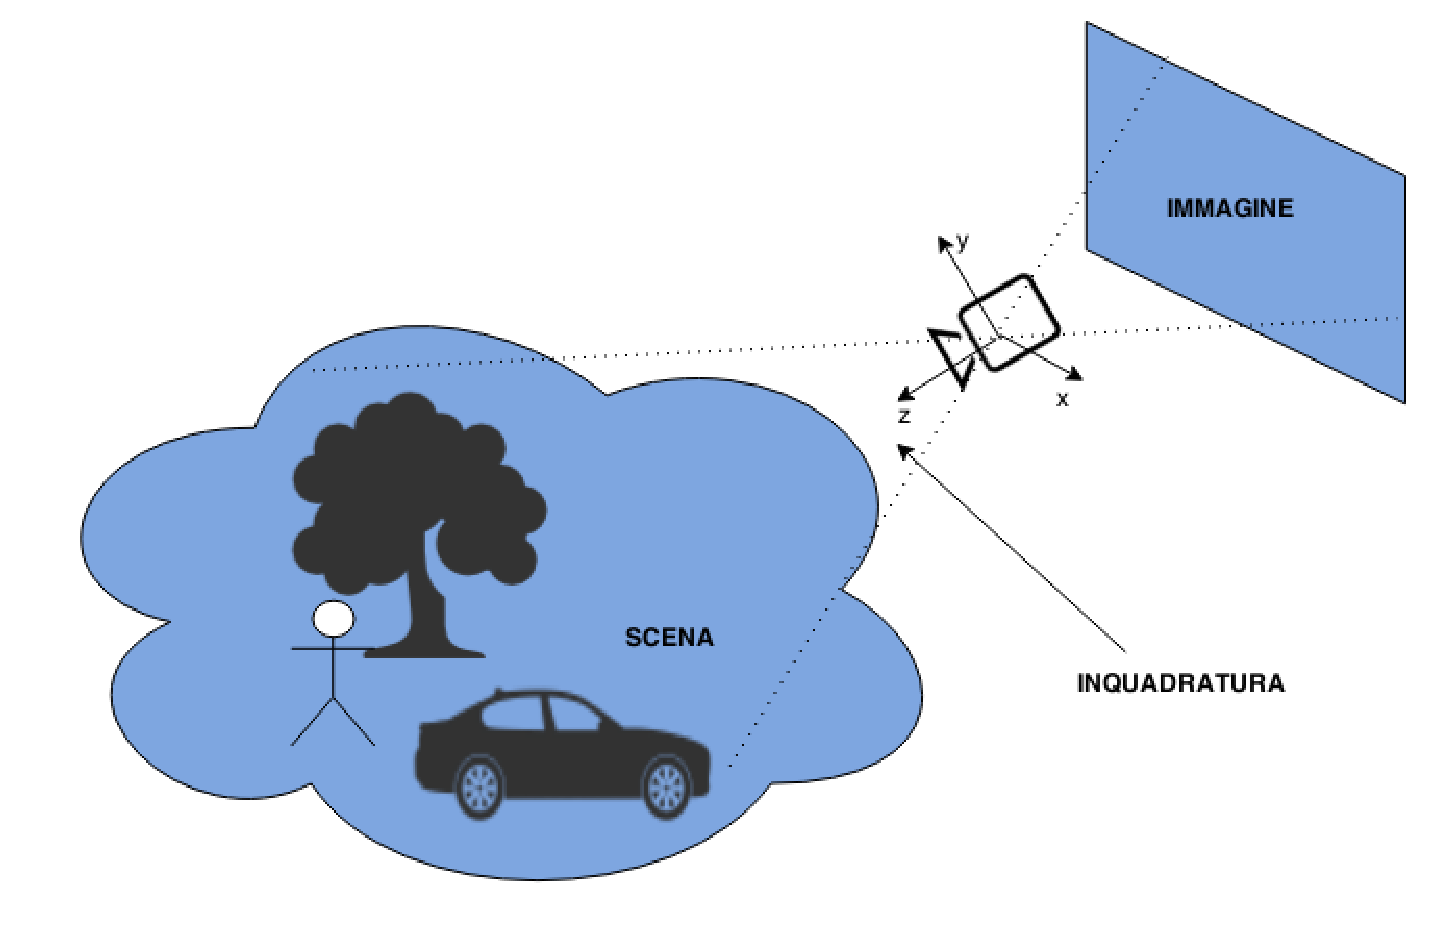
\includegraphics[width=12cm]{./pictures/videoMonitoring}
	\caption{Sistema di monitoraggio video}
	\label{fig:videoMonitoring}
\end{figure}
\noindent 
La posizione e la rotazione della camera determinano l'\textit{\gls{inquadratura}} della scena.
L'acquisizione, da parte della camera, della scena nell'istante di tempo $i$ viene definita \textit{immagine} o \textit{frame} i-esimo.
La figura \ref{fig:videoMonitoring} illustra questi concetti.\\
Nel seguito della trattazione useremo una specifica terminologia.
Indicheremo con $\mathcal{X}$ l'insieme dei \textit{pixel} costituenti l'immagine acquisita dalla camera,
\[ \mathcal{X} \subset \mathbb{N}^2, \]
e con $x \in \mathcal{X}$ il singolo pixel.
Quando vorremo considerare il frame acquisito all'istante di tempo $i$, useremo $z_i$, con $i=1,\dots , \infty$. 
In particolare, per indicare il valore della \textit{luminosit\`a} del pixel $x$ per il frame $i$-esimo, useremo il termine $z_i(x)$, con 
\[ z_i(x) \in [0, 255]. \]
\section{Tampering Detection}
In un'applicazione di monitoraggio video consideriamo che la camera, in condizioni di funzionamento ottimale, mantenga la stessa inquadratura nel tempo e che sia in grado di acquisire, in maniera nitida, tutti gli elementi di interesse presenti nella scena.
Definiamo \gls{tampering} un qualsiasi evento che determina un cambio di inquadratura o che non permette la corretta acquisizione di parte o totalit\`a della scena.
Possiamo classificare gli eventi di tampering in quattro categorie:
\begin{itemize}
	\item sfocature,
	\item spostamenti della camera,
	\item occlusioni dell'obiettivo,
	\item guasti della camera.
\end{itemize}
Nei moderni sistemi di videosorveglianza troviamo spesso algoritmi utilizzati per identificare particolari eventi all'interno della scena ripresa dalla camera. 
Ad esempio \`e possibile avere un software in grado di identificare le targhe delle automobili che superano il limite di velocit\`a, oppure la presenza di oggetti incustoditi in una stazione \cite{Targhe}.
Affinch\'e questi algoritmi funzionino correttamente, \`e importante che l'\textit{affidabilit\`a} del sistema di acquisizione sia preservata.
Per fare questo la letteratura scientifica offre molte tecniche che permettano l'identificazione automatica di eventi in grado di compromettere la corretta ripresa della scena da parte della videocamera.
Possiamo dividere le principali tecniche di tampering detection in due categorie: 
\begin{itemize}
	\item tecniche basate su confronto di background,
	\item tecniche basate su monitoraggio sequenziale.
\end{itemize}
\subsection{Tecniche basate su confronto di background}
Nella maggior parte dei lavori dedicati a questo problema, il concetto principale consiste nel confrontare ciascun frame con un modello che viene calcolato utilizzando i frame precedenti.
Tale modello \`e ampiamente utilizzato in vari ambiti di visione artificiale e prende il nome di \textit{modello di background}.
Un metodo generale di calcolo del background \`e presentato in \cite{aksay2007camera}.
Indichiamo con $z_i(x)$ il valore, nel pixel $x$, della luminosit\`a nell'$i$-esimo frame.
Il valore del modello di background \`e calcolato in maniera ricorsiva secondo la seguente formula:
\begin{equation}
\label{eq:background}
B_{i + 1}(x)=\left\{ \begin{array} {lcl}
aB_i(x)+ (1-a)z_i(x) & \mbox{, se} & |z_i(x) - z_{i-1}(x)|\leq T_i(x) \\
B_i(x) & \mbox{, se} & |z_i(x) - z_{i-1}(x)|>T_i(x)\end{array} \right. ,
\end{equation}
dove $0 < a < 1$ \`e chiamato \textit{parametro di aggiornamento} (\textit{update parameter}) e $T_i(x)$ \`e una soglia che permette di identificare un cambiamento sostanziale di luminosit\`a nel pixel $(x)$. 
 Questa soglia viene aggiornata in maniera ricorsiva secondo la seguente formula:
  \begin{equation}
  \label{eq:backgroundThreshUpd}
  T_{i + 1}(x)=\left\{ \begin{array} {lcl}
  aT_i(x)+ (1-a)(c |z_i(x) - B_i(x)|) & \mbox{, se} & |z_i(x) - z_{i-1}(x)|\leq T_i(x) \\
  T_i(x) & \mbox{, se} & |z_i(x) - z_{i-1}(x)|>T_i(x) \end{array} \right. ,
  \end{equation}
  dove $c > 1$ e $0<a<1$.
  Lo stesso modello viene applicato in altri lavori (\cite{saglam2009real}, \cite{tsesmelis2013tamper}), mentre una variante molto usata consiste nell'estrarre il modello di background a partire dall'\textit{estrazione dei contorni} da ciascun frame (\cite{harasse2004automated}, \cite{gil2007automatic}).
\subsubsection{Identificazione di occlusioni}
L'evento di occlusione avviene quando un oggetto opaco viene posto vicino alla camera, in modo da coprire la scena ripresa.
In \cite{aksay2007camera} e \cite{saglam2009real} questo evento \`e associato a un cambiamento nella struttura dell'\textit{istogramma} del frame occluso rispetto a quello del background.
Infatti, nel caso di occlusioni, i valori dell'istogramma tendono a concentrarsi in un intervallo molto ristretto, verso i livelli pi\`u bassi della scala di grigi.\\
Un approccio simile \`e presente in \cite{harasse2004automated}, \cite{gil2007automatic} e \cite{ellwart2012camera}, in cui l'evento di occlusione \`e associato a un abbassamento dell'\textit{entropia}:
 \begin{equation}
 \label{eq:entropy}
 E=-\sum_{k}p_k\ln(p_k) ,
 \end{equation}
 dove $p_k$ rappresenta la probabilit\`a che il livello di grigio $k$ sia presente all'interno dell'immagine. 
\subsubsection{Identificazione di spostamenti della camera}
Quando viene spostata la camera, in modo cambi l'inquadratura della scena, l'immagine di background $B_i$ viene lentamente aggiornato in modo da riflettere i cambiamenti avvenuti nei frame. 
In \cite{saglam2009real} il metodo proposto per identificare uno spostamento della camera consiste nel confrontare l'immagine di background $B_i$ con $B_{i-k}$, ovvero con un secondo modello \textit{ritardato} di $k$ frame, dove $k \in \mathbb{Z}^+$.
L'approccio consiste nel calcolare un \textit{valore di proporzione} $P$, ottenuto dal confronto tra i due modelli:
\begin{equation}
\label{eq:displEqSaglam}
P=\left\{ \begin{array} {lcl}
P+1 & \mbox{, se} & B_i(x) \neq B_{n-k}(x) \\
P & \mbox{, se} & B_i(x) = B_{n-k}(x) \end{array} \right. .
\end{equation}
Lo spostamento della camera viene identificato quando $P > Th K$, dove $0<Th<1$ \`e un valore di soglia scelto in base alla sensibilit\`a che si vuole dare all'algoritmo e $K$ \`e il numero totale di pixel dell'immagine.\\
Un altro approccio \`e quello di utilizzare tecniche di \textit{block matching}.
In \cite{gil2007automatic} e \cite{harasse2004automated} il confronto viene fatto utilizzando la formula \textit{zero-mean normalized cross correlation} (ZNCC) \cite{roma2002comparative}:
\begin{equation}
ZNCC_i(m) = \frac{\sum_{x \in \mathcal{X}}(B_{i-1}(x)- \mu_{B_{i-1}})(z_i(x+m)-\mu_{z_i})}{\sigma_{B_{i-1}} \sigma_{z_i}},
\end{equation} 
dove $\mu_{z_i}$ e $\sigma_{z_i}$ rappresentano la media e la deviazione standard della luminosit\`a nell'immagine $z_i$.
Un'altra cifra di merito, utilizzata in \cite{ellwart2012camera}, \`e la \textit{minimum squared difference} (MSD):
\begin{equation}
MSD = \frac{1}{K}\sum_{x \in \mathcal{X}}(z_i - B_i)^2
\end{equation}
L'algoritmo di block matching fornisce due parametri:
il primo parametro, $m$, indica il \textit{vettore della traslazione} tra il background e il frame corrente, mentre il secondo parametro \`e lo ZNCC relativo a quel vettore.
Lo spostamento viene individuato quando il vettore $m$ ha una lunghezza minima e lo ZNCC corrispondente supera una certa soglia.
Un metodo simile viene utilizzato anche in \cite{kryjak2012fpga}, con la differenza che, invece di analizzare la correlazione dei pixel, viene analizzata quella degli istogrammi. 
\subsubsection{Identificazione di sfocature} 
La conseguenza di un evento di sfocatura \`e la perdita di dettagli nell'immagine.
In \cite{aksay2007camera} e \cite{saglam2009real} questo fenomeno \`e associato a una diminuzione dell'energia ad alta frequenza. 
Per analizzare questo cambiamento, \cite{aksay2007camera} confronta ciascun frame con il background nel dominio delle \textit{wavelet} \cite{mallat1989theory}, mentre \cite{saglam2009real} utilizza il dominio della \textit{trasformata di Fourier} \cite{bracewell1978fourier}.
\begin{figure}
	\centering
	\begin{subfigure}[]
		{\label{fig:defocusNormale} 
\includegraphics[width = 5cm]{./pictures/normale}}
	\end{subfigure}
	\begin{subfigure}[]
		{\label{fig:defocusNormaleFourier} 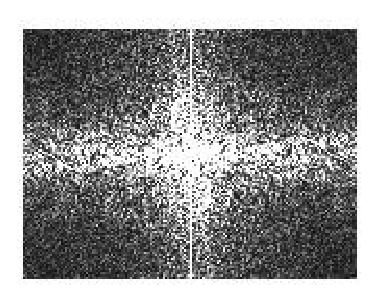
\includegraphics[width = 5cm]{./pictures/normale-fourier}}
	\end{subfigure}
	\begin{subfigure}[]
		{\label{fig:defocusSfocato} 
\includegraphics[width = 5cm]{./pictures/sfocato}}
	\end{subfigure}
	\begin{subfigure}[]
		{\label{fig:defocusSfocatoFourier} 
\includegraphics[width = 5cm]{./pictures/sfocato-fourier}}
	\end{subfigure}
	\caption{Comportamento della trasformata di Fourier nel caso di sfocatura}
	\label{fig:fourier}
\end{figure}
Nella figura \ref{fig:fourier} vediamo un esempio di come si comporta la trasformata di Fourier nel caso di sfocature: 
nel passaggio da un frame nitido (Fig. \ref{fig:defocusNormale}) a uno sfocato (Fig. \ref{fig:defocusSfocato}) abbiamo un crollo delle componenti ad alta frequenza nelle trasformate di Fourier (rispettivamente Fig. \ref{fig:defocusNormaleFourier} e Fig. \ref{fig:defocusSfocatoFourier}).
L'evento di tampering viene individuato quando l'\textit{energia media} della trasformata di Fourier (o di quella wavelet) del frame corrente $E_{HF}(z_i)$ \`e $Th$ volte minore di quella del background $E_{HF}(B_i)$:
\[E_{HF}(z_i)\leq Th E_{HF}(B_i),\]
dove $0<Th<1$ \`e  un valore di soglia scelto in base alla sensibilit\`a che si vuole dare all'algoritmo.\\
Un altro approccio consiste nell'analizzare la perdita di dettagli confrontando i contorni (\textit{edges}) del frame corrente con quelli del background.
Questo metodo, utilizzato in \cite{ellwart2012camera}, \cite{gil2007automatic}, \cite{harasse2004automated} e \cite{kryjak2012fpga}, consiste nell'estrarre i contorni dalle immagini secondo il metodo di Sobel \cite{sobel19683x3} o di Canny \cite{canny1986computational}, e confrontare il numero di pixel dei contorni con quelli del background. 
Quando il numero di pixel dei contorni del frame corrente $\sum edges(z_i)$ \`e $Th$ volte pi\`u piccolo di quello del background $\sum edges(B_i)$:
\[ \sum edges(z_i) \leq Th \sum edges(B_i), \]
dove $0<Th<1$ \`e  un valore di soglia scelto in base alla sensibilit\`a che si vuole dare all'algoritmo.
\subsection{Tecniche basate su monitoraggio sequenziale}
\chapter{Impostazione del problema di ricerca}
\label{FormulazioneProblema}
\thispagestyle{empty}

%\begin{quotation}
%{\footnotesize
%\noindent{\emph{``Terence: Rotta a nord con circospezione \\
%Bud: Ehi, gli ordini li do io qui!\\
%Terence: Ok, comante\\
%Bud: Rotta a nord\\
%Terence: Soltanto?\\
%Bud: Con circospezione!''}
%}
%\begin{flushright}
%Chi Trova un Amico Trova un Tesoro
%\end{flushright}
%}
%\end{quotation}
\vspace{0.5cm}
In questo capitolo descriviamo il problema, affrontato dall'algoritmo di tampering detection, in maniera formale e rigorosa. Il primo paragrafo illustra il modello delle osservazioni e gli eventi che siamo interessati a identificare, mentre il secondo paragrafo formalizza il concetto di tampering detection. 
\noindent 
\section{Modello delle osservazioni}
Il nostro campo di osservazione si concentra su quegli eventi che si interpongono tra la scena ripresa da una camera e il sensore che acquisisce le immagini. Non vogliamo, cio\`e, identificare degli eventi particolari che avvengono nella scena, come un oggetto lasciato incustodito \cite{Targhe}, bens\`i vogliamo identificare quegli eventi tali per cui il sensore non \`e pi\`u nelle condizioni di riprendere, in maniera ottimale, la scena, quali ad esempio sfocature o spostamenti della camera.
Nel seguito cerchiamo di dare una definizione formale di questi eventi.
\subsection{Scena e posizione della camera}
Prima di tutto definiamo, in maniera rigorosa, i termini che verranno utilizzati nel seguito della trattazione.\\
Lo scenario che consideriamo \`e quello di una camera che deve riprendere una particolare \textit{\gls{scena}}.
La posizione e la rotazione della camera determinano l'\textit{\gls{inquadratura}} della scena.
In un'applicazione di monitoraggio video consideriamo che la camera, in condizioni di funzionamento ottimale, mantenga la stessa inquadratura nel tempo e che si in grado di acquisire, in maniera nitida, tutti gli elementi di interesse presenti nella scena.
Definiamo \gls{tampering} un qualsiasi evento che determina un cambio di inquadratura o che non permette la corretta acquisizione di parte o totalit\`a della scena.
Possiamo classificare gli eventi di tampering in quattro categorie:
\begin{itemize}
	\item Sfocature
	\item Spostamenti della camera
	\item Occlusioni
	\item Guasti della camera
\end{itemize}

\subsection{Sfocatura}
Il fenomeno della sfocatura avviene quando un elemento trasparente o semitrasparente si interpone tra la lente della camera e la \gls{scena} ripresa, oppure quando viene cambiata la messa a fuoco, causando una perdita nei dettagli della \gls{scena} ripresa.

\begin{figure}
	\centering
	\begin{subfigure}[Pioggia sull'obiettivo]
		{\label{fig:pioggia} 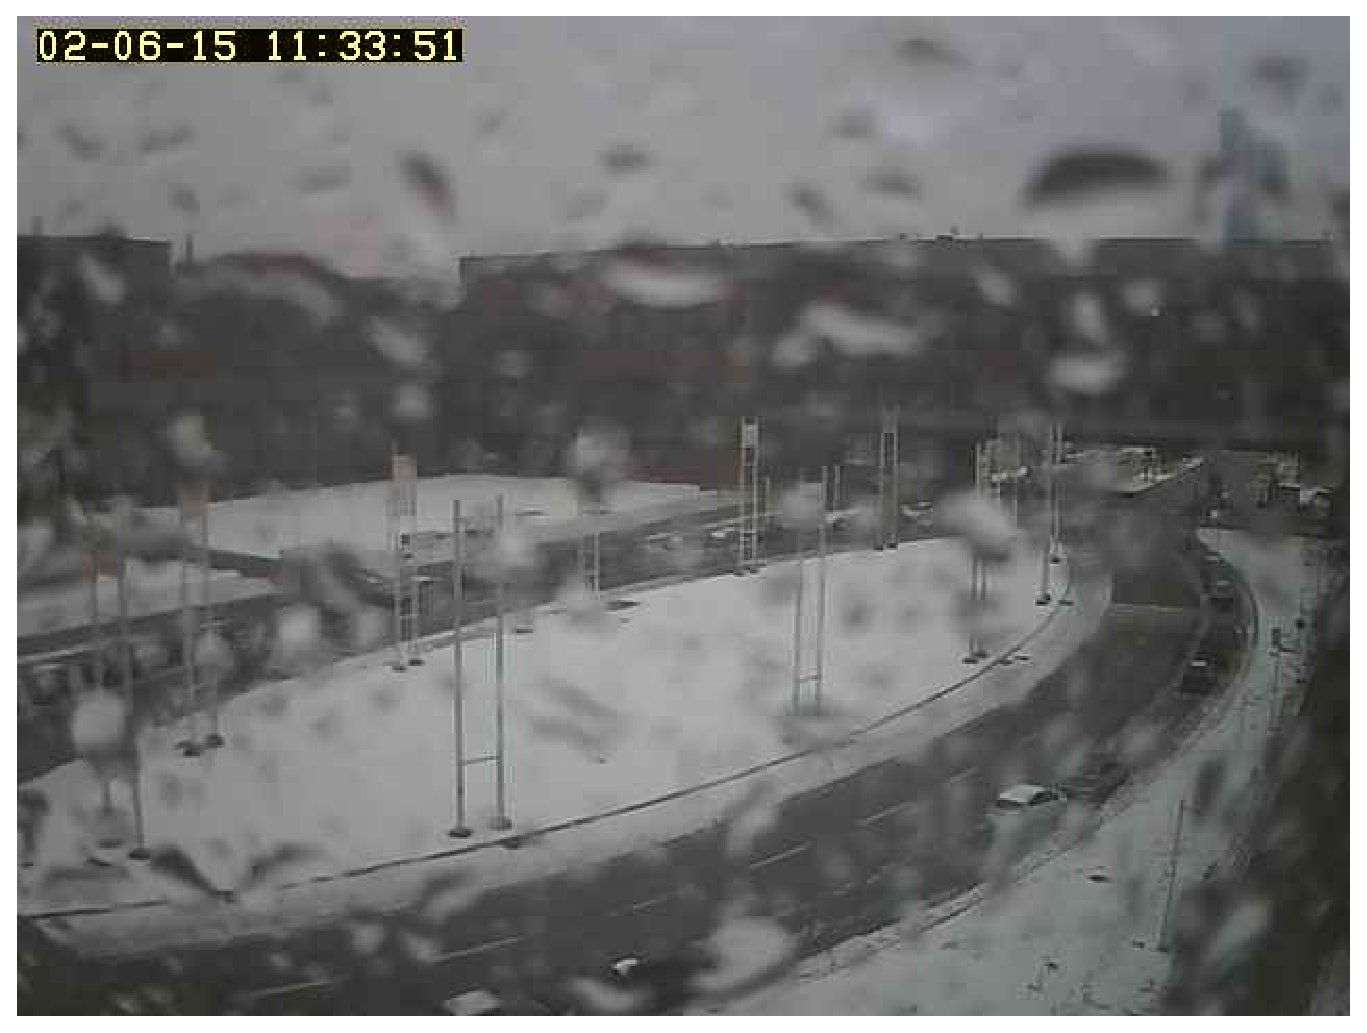
\includegraphics[width=6cm]{./pictures/pioggia}}
	\end{subfigure}
	\begin{subfigure}[Deodorante spray]
		{\label{fig:bassiniDEFOCUS} \includegraphics[width=6cm]{./pictures/bassiniDEFOCUS}}
	\end{subfigure}
	\caption{Esempi di sfocature}
	\label{fig:esempiSfocature}
\end{figure}

\noindent Nella figura \ref{fig:esempiSfocature} sono mostrati degli esempi in cui sono presenti delle sfocature. 
Queste possono essere di origine diversa: 
\begin{itemize}
	\item dovute a \textit{cause naturali}, come ad esempio dell'acqua piovana che si deposita sulla lente (figura \ref{fig:pioggia}), o la condensa dovuta all'umidit\`a e alle basse temperature, oppure un raggio di sole incidente sull'obiettivo della camera;
	\item per \textit{intervento dell'uomo}, che a sua volta pu\`o avvenire in maniera intenzionale (e in questo caso si pu\`o parlare di \textit{manomissione}) oppure non intenzionale. Ad esempio, si pu\`o direttamente intervenire sulla messa a fuoco, nel caso sia possibile cambiarla manualmente; oppure (come nel caso della figura \ref{fig:bassiniDEFOCUS}) \`e possibile applicare una sostanza semitrasparente sulla lente della camera, come il gas di un deodorante spray.
\end{itemize}
Riprendendo \cite{alippi2010detecting}, questo fenomeno pu\`o essere modellato come un operatore di \textit{degradazione} $D$ applicato a un'immagine $y$, considerata priva di errori, i.e.,
\begin{equation}
z=\mathcal{D}[y].
\end{equation}
In particolare, all'interno dell'operatore $\mathcal{D}$ si pu\`o considerare il contributo dovuto a un operatore di \textit{sfocatura} $B$ (dall'inglese \textit{blur}) e un termine aleatorio $\eta$ corrispondente al rumore, i.e.,
\begin{equation}
\label{blur_single}
z(x)=\mathcal{D}[y](x) = \mathcal{B}[y](x) + \eta(x), \qquad x \in \mathcal{X}
\end{equation}
dove abbiamo indicato con $x$ le coordinate dei \textit{pixel} dell'immagine e $\mathcal{X}$ \`e l'insieme dei pixel che formano l'immagine. 
Considerando il caso continuo, possiamo assumere la sfocatura $\mathcal{B}$ come un operatore \textit{lineare},
\begin{equation}
\mathcal{B}[y](x) = \int_{\mathcal{X}}y(s)h(x,s)ds,
\end{equation}
dove $h(x,s)$ rappresenta la \textit{risposta all'impulso} (\textit{point spread function} (PSF)) della sfocatura sul pixel $x$, il cui risultato consiste nel rendere le differenze di intensit\`a, tra pixel adiacenti, pi\`u morbide (\textit{smooth}).
Nel caso in cui la sfocatura sia applicata sulla totalit\`a dell'immagine (come nel caso della figura \ref{fig:bassiniDEFOCUS}), allora \`e possibile modellare l'operatore di blur come una \textit{convoluzione}\footnote{Il blur convoluzionale \`e quello che abbiamo utilizzato per generare, in maniera sintetica, sequenze con immagini sfocate.}:
\begin{equation}
\label{blur_convolution}
\mathcal{B}[y](x) = \int_{\mathcal{X}}y(s)h(s-x)ds,
\end{equation}
dove $h(.)$ \`e un filtro gaussiano o uniforme.\\
Nel caso pi\`u generale possiamo considerare che la camera acquisisca un sequenza di $N$ osservazioni $\{z_i\}, i = 1, \dots ,N$, quindi la formula \ref{blur_single} si pu\`o riscrivere come
\begin{equation}
\label{blur_multi}
z_i(x)=\mathcal{D}_i[y_i](x) = \mathcal{B}_i[y_i](x) + \eta(x), \qquad x \in \mathcal{X}.
\end{equation}

La sequenza delle immagini $\{y_i\}, i = 1,\dots , N$, pu\`o variare in maniera significativa nel suo contenuto, anche nel caso in cui la vista sia la stessa.
\begin{figure}
	\centering
	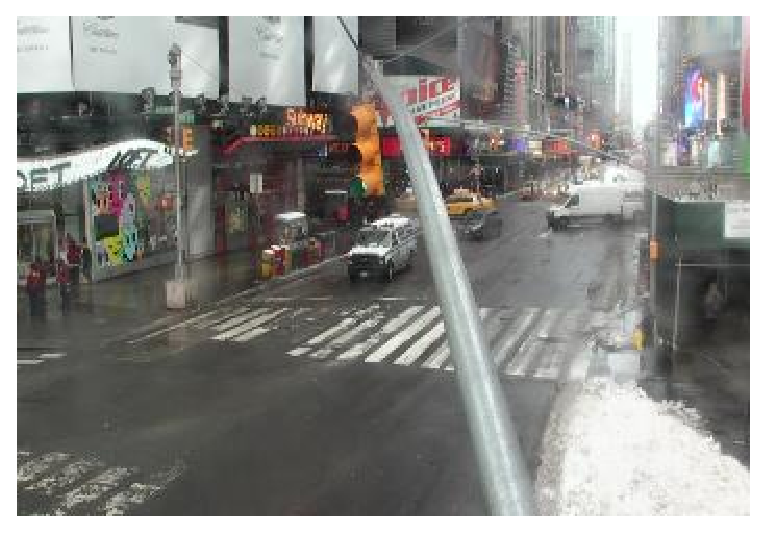
\includegraphics[width=3cm]{./pictures/image0001.eps}
	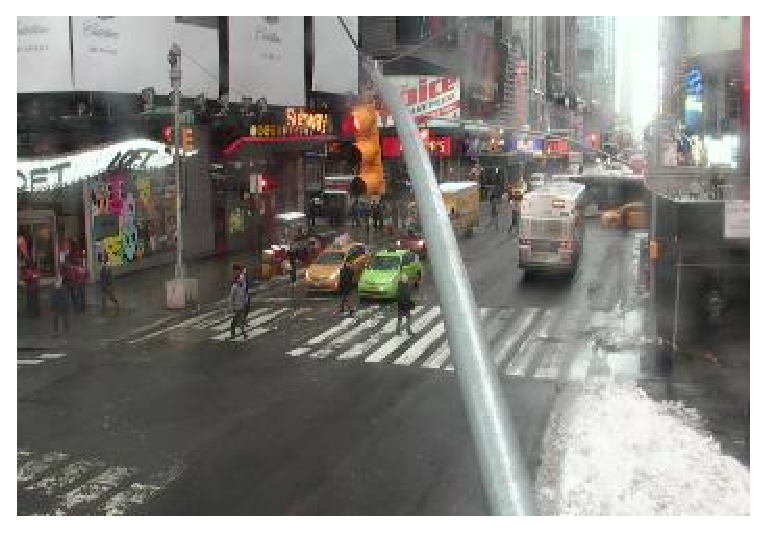
\includegraphics[width=3cm]{./pictures/image0002.eps}
	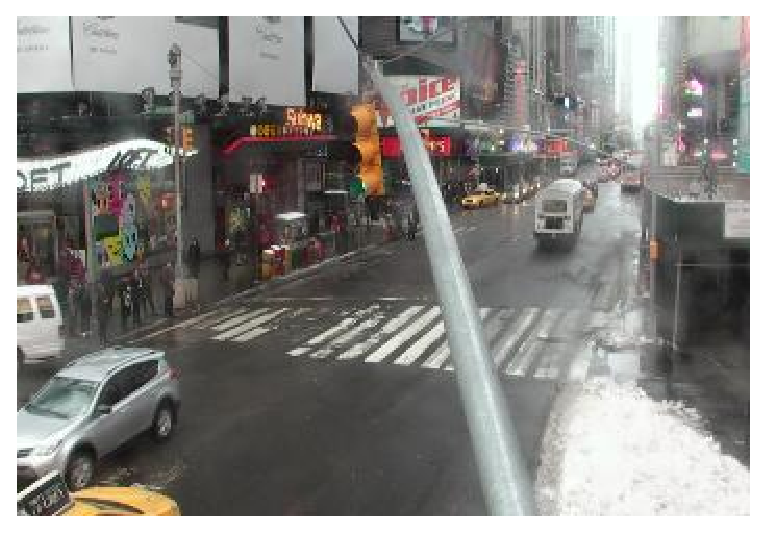
\includegraphics[width=3cm]{./pictures/image0003.eps}
	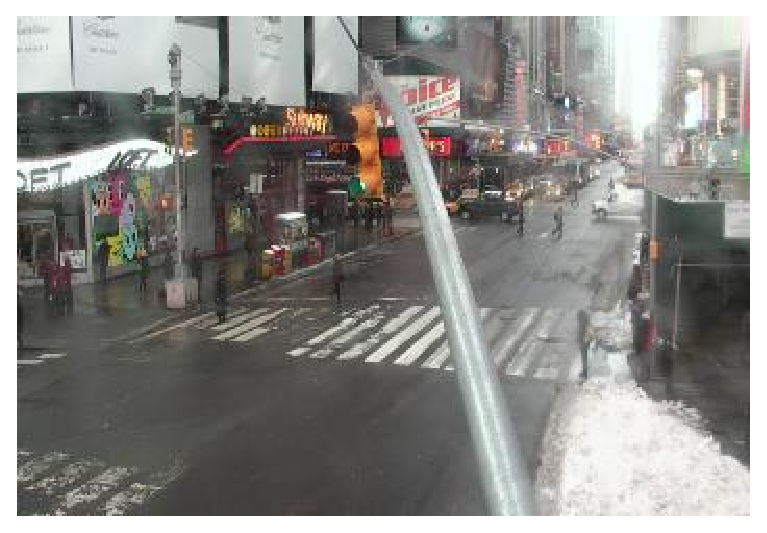
\includegraphics[width=3cm]{./pictures/image0004.eps}
	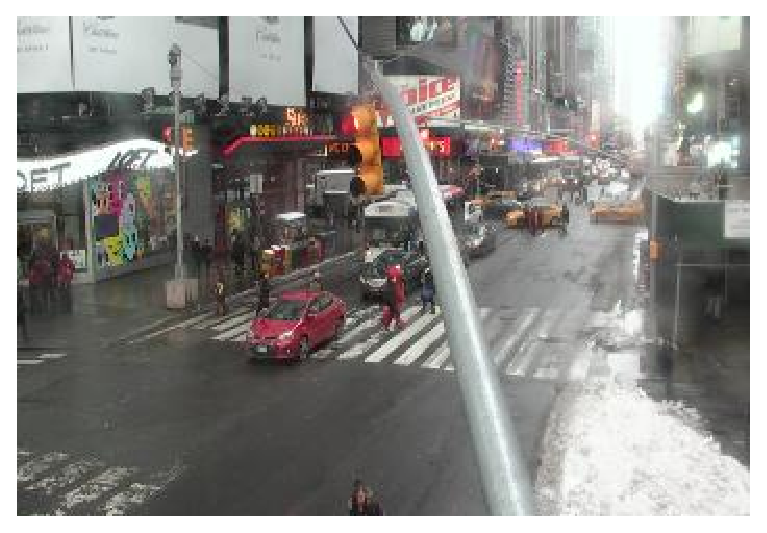
\includegraphics[width=3cm]{./pictures/image0005.eps}
	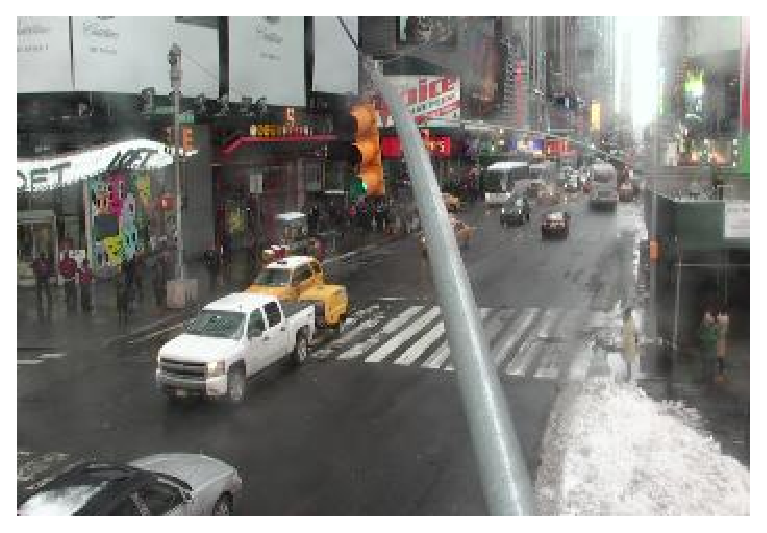
\includegraphics[width=3cm]{./pictures/image0006.eps}
	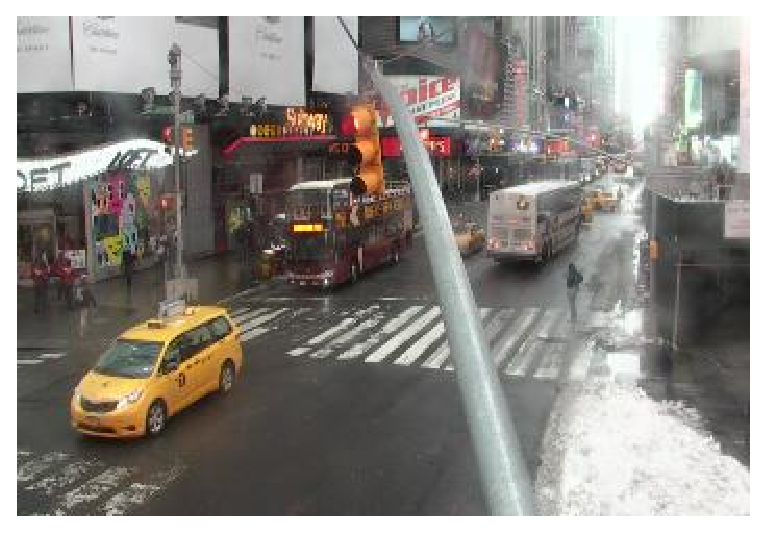
\includegraphics[width=3cm]{./pictures/image0007.eps}
	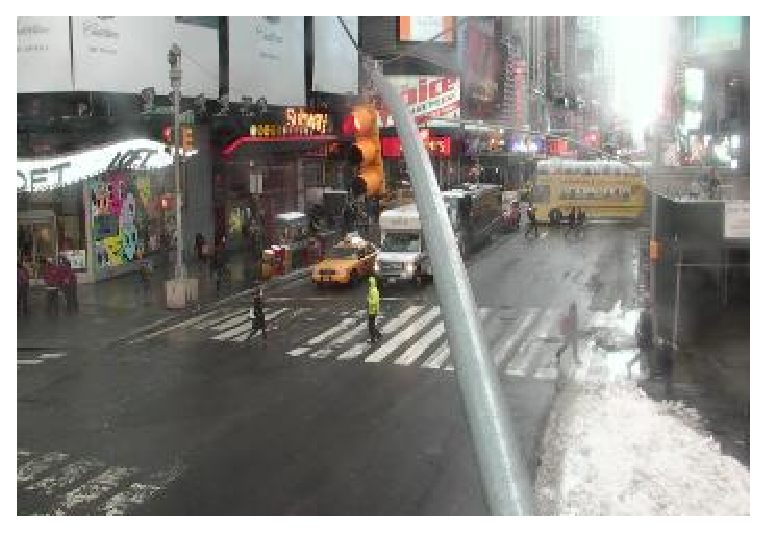
\includegraphics[width=3cm]{./pictures/image0008.eps}
	\caption{Sequenza di otto frame consecutivi acquisiti ogni minuto}
	\label{fig:framDifferences}
\end{figure}
\noindent Un esempio \`e illustrato nella figura \ref{fig:framDifferences}, in cui le immagini riprese dalla camera sono acquisite ogni minuto. 
Nonostante l'inquadratura non cambi tra le acquisizioni, il contenuto delle singole immagini varia parecchio, dato il continuo passaggio di automobili e pedoni.
Questo problema fa s\`i che l'identificazione delle sfocature non possa avvenire facendo un semplice confronto tra frame consecutivi, in quanto avremmo un numero troppo elevato di falsi positivi.
Infatti, nel caso in cui avessimo un riscontro negativo dal confronto tra due frame ($z_i \neq z_{i + 1}$), sarebbe difficile capire se \`e cambiato il contenuto delle immagini ($y_i \neq y_{i + 1}$) o l'operatore di sfocatura ($\mathcal{B}_i \neq \mathcal{B}_{i + 1}$). 
\subsection{Spostamento della camera}
Lo spostamento della camera avviene quando cambia la sua vista.
Le cause possono essere, ancora una volta, di tipo naturale, ad esempio una raffica di vento che sposta la camera, oppure dovute a un intervento malevolo da parte di un uomo.
\begin{figure}
	\centering
	\subfigure[Vista originale]{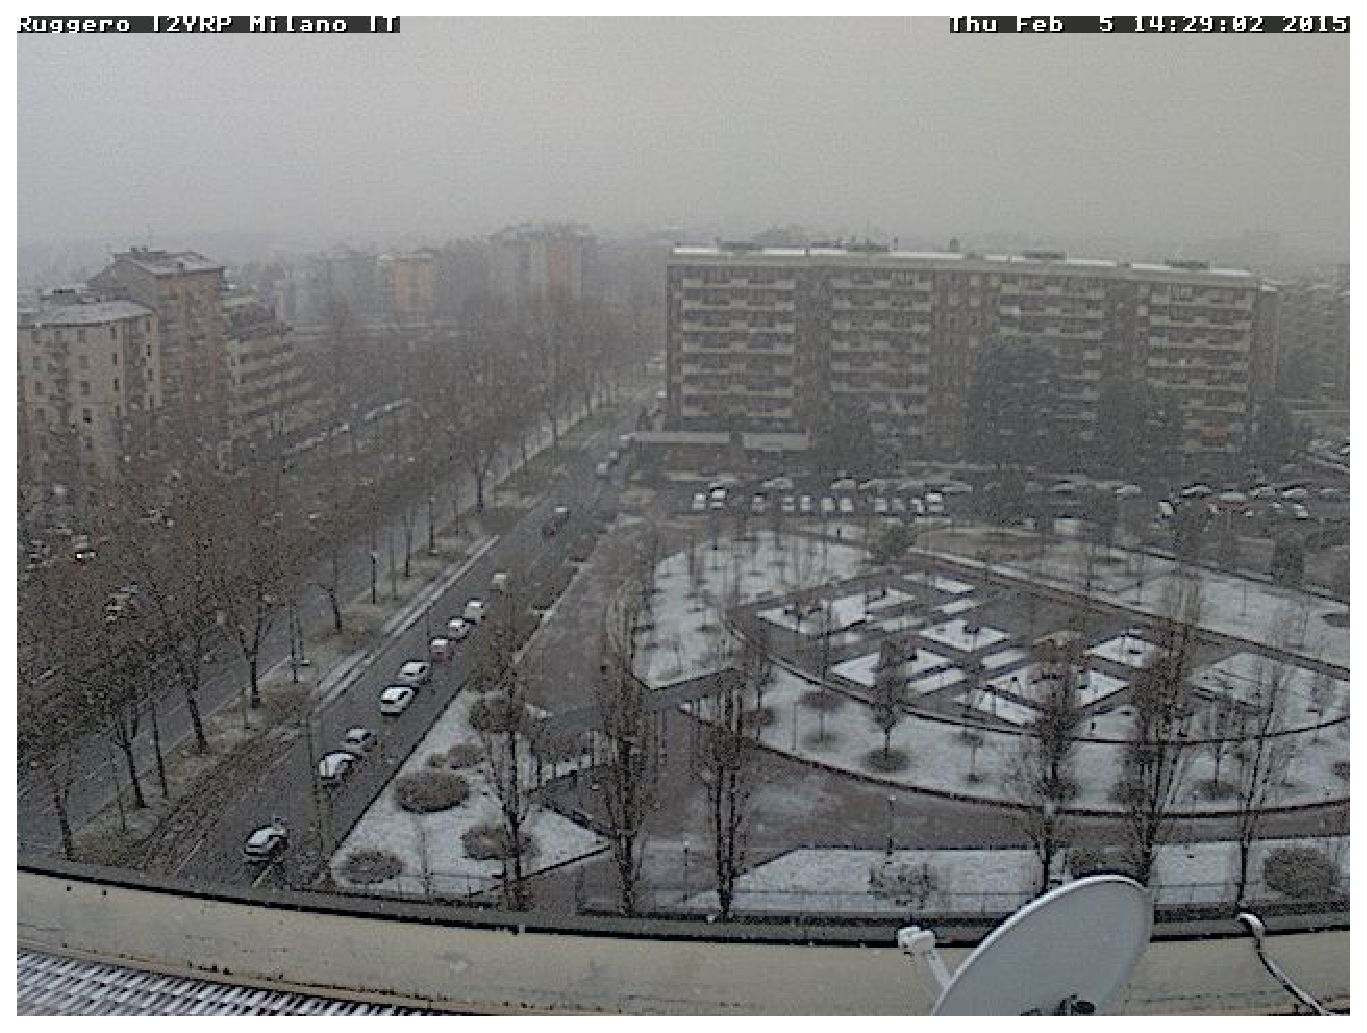
\includegraphics[width=6cm]{./pictures/testiORIGINALE}}
	\subfigure[Vista in seguito allo spostamento della camera]{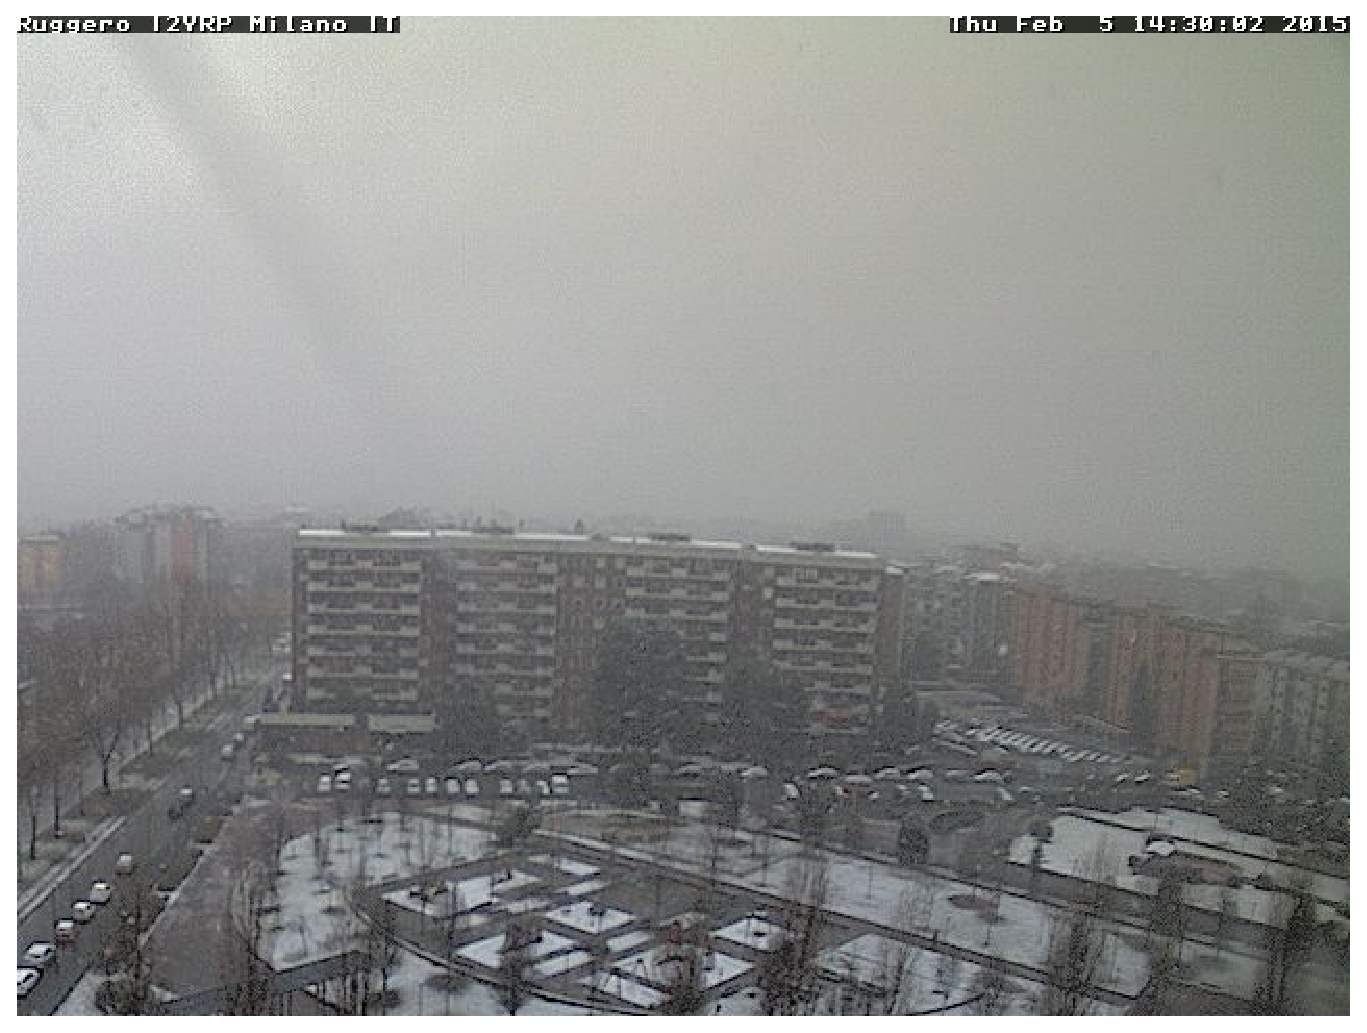
\includegraphics[width=6cm]{./pictures/testiDISPLACEMENT}}
	\caption{Esempio di spostamento della camera}
	\label{fig:testiDISPLACEMENT}
\end{figure}
\noindent Un esempio di spostamento della camera \`e mostrato nella figura \ref{fig:testiDISPLACEMENT}.
Possiamo formalizzare il concetto di spostamento della camera nel modo seguente: consideriamo la sequenza $\{y_i\}$ di immagini generate da una camera in una certa posizione, e la sequenza $\{w_i\}$ di immagini generate dalla stessa camera in una posizione differente.\\
Possiamo, dunque, considerare la sequenza di immagini $\{z_i\}$ in cui avviene uno spostamento della camera all'istante $T^*$ nel seguente modo:
\begin{equation}
\label{eq:displacement}
z_i(x) = \mathcal{S}_i[y_i](x) = \left\{ \begin{array}{rcl}
	y_i(x) + \eta(x) & \mbox{per} & i < T^* \\
	w_i(x) + \eta(x) & \mbox{per} & i \geqslant T^*
	\end{array}\right. ,
\end{equation}
dove $\eta(x)$ \`e un rumore stazionario.\\
In questa formulazione abbiamo considerato lo spostamento come un fenomeno \textit{istantaneo};
in generale, possiamo considerare una fase \textit{transitoria} in cui l'inquadratura della camera cambia a ogni \gls{frame} acquisito, fino a raggiungere la posizione finale. 
Dato che, nella nostra applicazione, la camera opera con \gls{framerate} bassi (come ad esempio un'immagine al minuto), possiamo considerare lo spostamento come istantaneo e, quindi, tenere come riferimento il modello della formula \ref{eq:displacement}.\\
%Nella formulazione pi\`u generale possiamo, quindi, assumere un istante $T_{start}^ *$ in cui inizia lo spostamento e un istante $T_{end}^*$ in cui termina il transitorio:
%\begin{equation}
%\label{eq:displacementGeneral}
%z_i(x) = \left\{ \begin{array}{rcl}
%y_i(x) + \eta(x) & \mbox{per} & i < T_{start}^* \\
%v_i(x) + \eta(x) & \mbox{per} & T_{start}^* \leq i < T_{end}^* \\
%w_i(x) + \eta(x) & \mbox{per} & i \geqslant T_{end}^*
%\end{array}\right. ,
%\end{equation}
%dove $\{v_i\}$ rappresenta la sequenza di immagini generate da viste differenti.
%Inoltre, durante il transitorio dello spostamento, il tempo di esposizione della camera pu\`o portare alla generazione di sfocature nelle immagini.\\
Anche per lo spostamento della camera vale la considerazione fatta nel caso della sfocatura: il contenuto delle immagini varia con il passare del tempo, quindi identificare lo spostamento confrontando frame consecutivi nel tempo genera un alto numero di falsi positivi.
\subsection{Occlusione e guasti della camera}
Il fenomeno dell'occlusione avviene quando un oggetto opaco si pone a ridosso della camera, impedendo la visione di una parte, se non la totalit\`a, della scena. 
L'effetto di questo evento \`e quello di impedire l'acquisizione della scena nella sua totalit\`a.
Un esempio di occlusione ce l'abbiamo quando qualcuno copre la camera con un cappello, o mette un foglio di giornale davanti alla lente del sensore, oppure pu\`o succedere che della neve si accumuli sull'ottica del sensore.
\begin{figure}
	\centering
	\subfigure[Occlusione volontaria]{\label{fig:occlusionCALZA} 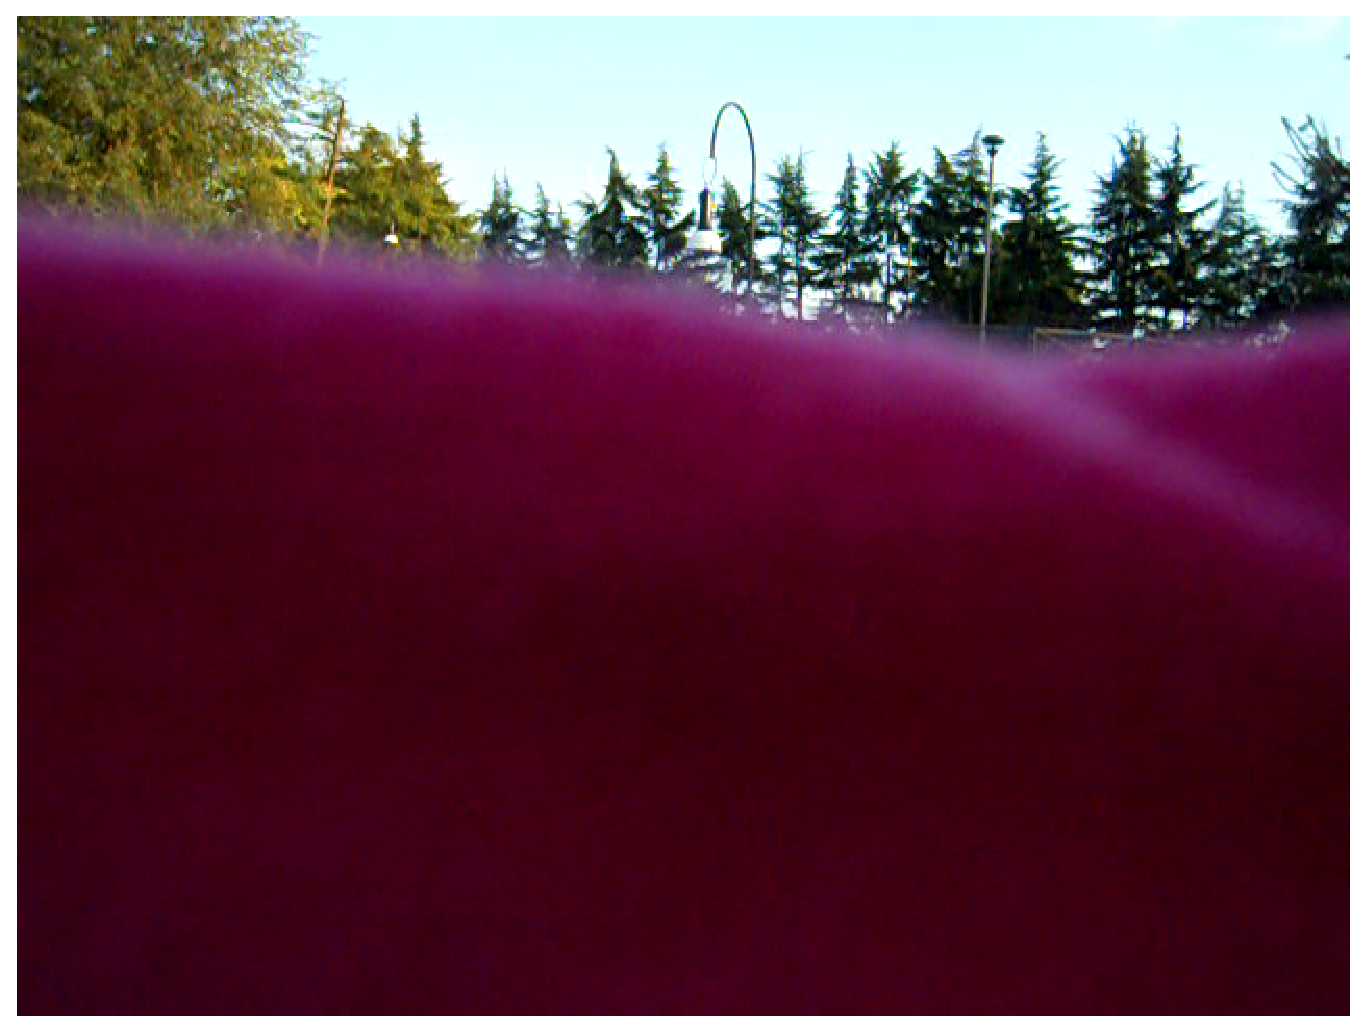
\includegraphics[width=6cm]{./pictures/calza}}
	\subfigure[Occlusione dovuta a deposito di neve]{\label{fig:occlusionNEVE}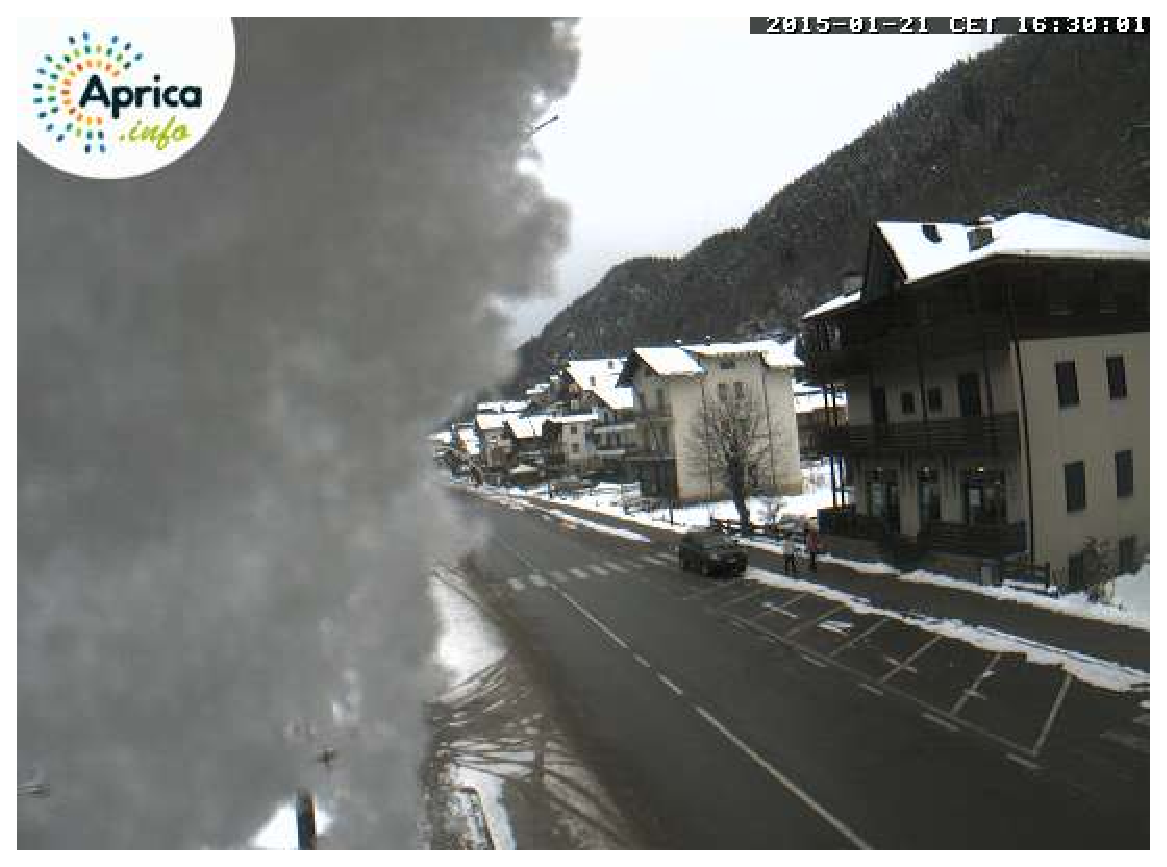
\includegraphics[width=6cm]{./pictures/neve}}
	\caption{Esempi di occlusione}
	\label{fig:occlusion}
\end{figure}
\noindent Il guasto del sensore invece comporta un aumento del rumore presente nell'immagine. \\
Queste problemi non sono stati affrontati durante la tesi, comunque le tecniche messe a punto per rilevare spostamenti e sfocature possono essere utilizzate anche per rilevare questo tipo di eventi. 
\section{Tampering detection}
L'algoritmo di tampering detection consiste nell'analizzare la sequenza di osservazioni $\{z_i\}, i=1, \dots , N$ in modo da determinare un possibile cambiamento nell'operatore di degradazione $\mathcal{D}$ o in quello di spostamento $\mathcal{S}$.
Come abbiamo illustrato precedentemente, discriminare tra cambiamenti avvenuti a livello di contenuto della scena e cambiamenti dovuti a tampering pu\`o diventare complicato confrontando direttamente i frame tra loro.
\chapter{Soluzione proposta}
\label{SoluzioneProposta}
\thispagestyle{empty}

%\begin{quotation}
%{\footnotesize
%\noindent{\emph{``Terence: Rotta a nord con circospezione \\
%Bud: Ehi, gli ordini li do io qui!\\
%Terence: Ok, comante\\
%Bud: Rotta a nord\\
%Terence: Soltanto?\\
%Bud: Con circospezione!''}
%}
%\begin{flushright}
%Chi Trova un Amico Trova un Tesoro
%\end{flushright}
%}
%\end{quotation}
\vspace{0.5cm}

\noindent
\section{Estrazione dei descrittori del cambiamento}
\section{Algoritmo di segmentazione}
\section{Monitoraggio one-shot}
\section{Monitoraggio sequenziale}
%\chapter{Architettura del sistema}
\label{Segmentazione}
\thispagestyle{empty}

%\begin{quotation}
%{\footnotesize
%\noindent{\emph{``Terence: Rotta a nord con circospezione \\
%Bud: Ehi, gli ordini li do io qui!\\
%Terence: Ok, comante\\
%Bud: Rotta a nord\\
%Terence: Soltanto?\\
%Bud: Con circospezione!''}
%}
%\begin{flushright}
%Chi Trova un Amico Trova un Tesoro
%\end{flushright}
%}
%\end{quotation}
\vspace{0.5cm}

\noindent 

\chapter{Realizzazioni sperimentali e valutazione}
\label{ProveSperimentali}
\thispagestyle{empty}

\vspace{0.5cm}

\noindent In questo capitolo illustriamo come sono stati condotti gli esperimenti per la valutazione del nostro algoritmo di tampering detection.
La prima parte \`e dedicata alla descrizione dei dataset utilizzati come riferimento, mostrando quali sistemi di acquisizione sono stati utilizzati e quali sono le metriche che abbiamo tenuto in considerazione.
Nella seconda parte, invece, entriamo nel dettaglio su quali sono stati i risultati a valle di tutta l'analisi sperimentale. 
\section{Acquisizione dei dataset}
Durante lo svolgimento della tesi abbiamo realizzato alcuni sistemi di acquisizione, in modo da avere un insieme di dataset (\textit{benchmark}) molto ampio che comprendesse sequenze video con diverse qualit\`a dei frame e con diversi framerate.
Alcune di queste sequenze sono state utilizzate per testare l'algoritmo di segmentazione, mentre altre hanno verificato l'algoritmo di tampering detection.
In generale, per ogni scena ripresa (dove per scena intendiamo una specifica inquadratura che \textit{non cambia} per le varie sequenze) abbiamo:
\begin{itemize}
	\item almeno una sequenza in cui non avviene nessun evento di tampering, che viene utilizzata per la creazione della mappa;
	\item almeno una sequenza in cui la camera subisce una sfocatura;
	\item almeno una sequenza in cui la camera subisce uno spostamento.
\end{itemize}
\subsection{Sistemi di acquisizione utilizzati}
\subsubsection{Camere ST}

\subsubsection{Raspberry Pi Camera}
Il sistema di acquisizione realizzato con le camere di ST aveva il problema di dover essere alimentato dalla rete elettrica.
Non \`e stato possibile, quindi, utilizzarlo per acquisizioni all'esterno.\\
Per ovviare a questo problema abbiamo deciso di realizzare un altro sistema basato su un \textit{Raspberry Pi modello B+} \cite{raspberry} con relativo \textit{modulo camera} \cite{raspberryCamera}.
Il Raspberry Pi \`e un \textit{single-board computer} (ovvero un computer implementato su una singola scheda elettronica) basato su un \textit{system-on-chip} (SoC) \textit{Broadcom BCM2835} \cite{broadcom}, che incorpora un processore \textit{ARM1176JZF-S} \cite{arm}, una GPU \textit{VideoCore IV} \cite{gpu} e $512$ MB di memoria.
Utilizza un sistema operativo \textit{Debian Linux} realizzato per processori ARM chiamato \textit{Raspbian} \cite{raspbian}.
Le ridotte dimensioni e il basso consumo di potenza hanno permesso di utilizzarlo per fare delle acquisizioni in ambienti esterni, utilizzando una batteria. 
\subsubsection{Estrazione frame dal web}

\subsection{Sequenze con presenza di tampering}
\subsection{Definizione dei ground thruth}
\subsection{Definizione delle metriche per la stima delle prestazioni}
\section{Risultati ottenuti}
\chapter{Conclusioni e direzioni future di ricerca}
\label{Conclusioni}
\thispagestyle{empty}

\noindent In questo lavoro di tesi abbiamo presentato una soluzione al problema, nei sistemi di monitoraggio video, di identificare particolari eventi che possano compromettere la corretta ripresa della scena, a cui si fa riferimento con il termine tampering.
In particolare abbiamo considerato l'utilizzo di camere intelligenti alimentate a batteria e lo scenario in cui la frequenza di acquisizione delle immagini da parte del sensore sia bassa, ad esempio un frame ogni minuto.\\
Abbiamo visto come il fatto di considerare dei framerate bassi complichi l'identificazione di eventi di tampering, in quanto le differenze tra frame consecutivi sono molto pi\`u elevate rispetto al caso di acquisizione continua. 
Inoltre, il fatto di avere algoritmi a bassa complessit\`a computazionale non ci permette di utilizzare degli indicatori troppo onerosi da estrarre dalle immagini.\\
La soluzione che abbiamo proposto \`e stata di utilizzare degli indicatori semplici, da estrarre in specifiche regioni della scena inquadrata dalla camera, e di monitorarli nel tempo con tecniche one-shot e sequenziali, in modo da individuare cambiamenti nel loro comportamento associabili a eventi di tampering.
Le regioni vengono estratte da un algoritmo di segmentazione della scena, che viene eseguito prima della messa in opera del sistema.\\
Abbiamo visto, infine, come le prove sperimentali condotte abbiano dimostrato che l'utilizzo della segmentazione della scena porti a dei miglioramenti nelle prestazioni dell'algoritmo, diminuendo il numero di falsi allarmi, senza aggiungere complessit\`a computazionale.
Un monitoraggio sequenziale sulla varianza dell'energia media del gradiente, inoltre, ha permesso di diminuire ulteriormente i falsi allarmi nell'identificazione degli eventi di sfocatura.\\
Gli sviluppi futuri riguarderanno il miglioramento dell'algoritmo e la sua integrazione su un dispositivo.
Per quanto riguarda l'identificazione di sfocature la ricerca dovr\`a essere condotta su come combinare il monitoraggio sequenziale con quello one-shot.
Per come \`e stato realizzato l'algoritmo al momento, infatti, le due tecniche sono eseguite in cascata, e il primo che identifica un cambiamento solleva l'allarme.
Dato che CONTINUARE!!!\\
Per quanto riguarda l'identificazione di spostamenti della camera un ulteriore sviluppo potrebbe riguardare l'integrazione delle informazioni estratte dalle immagini della camera con i dati estratti da dispositivi MEMS (\textit{Micro Electro-Mechanical Systems}), come \textit{sensori inerziali} o \textit{giroscopi}, in modo da poter validare gli allarmi ricevuti dalla camera e, quindi, ridurre ulteriormente i falsi allarmi.






%\appendix

%\pagestyle{fancy} 
%\fancyfoot{}                                               
%\renewcommand{\chaptermark}[1]{\markboth{\appendixname\ \thechapter.\ #1}{}} 
%\renewcommand{\sectionmark}[1]{\markright{\thesection.\ #1}}         
%\fancyhead[LE,RO]{\bfseries\thepage}    
                                        
%\fancyhead[RE]{\bfseries\leftmark}    
%\fancyhead[LO]{\bfseries\rightmark}     
%\renewcommand{\headrulewidth}{0.3pt} 

%\include{appendiceA}
%\include{appendiceB}
%\include{appendiceC}
%\include{appendiceD}
%\include{appendiceE}
%\include{appendiceF}

\backmatter
\cleardoublepage
% ---- Bibliography ----
\addcontentsline{toc}{chapter}{Bibliografia}
\bibliographystyle{plain}
\bibliography{bibl_tesi}
%\nocite{*}

%\printindex

\end{document}





